\chapter{Easter Koulourakia}
\label{ch:easter_koulourakia}
\index{dessert}
\index{cookies}
\index{Easter}

\marginnote{
    \textbf{Makes 45 cookies} \\
    Prep time: 20-30 minutes \\
    Cook time: 12-15 minutes \\
    \vspace*{\baselineskip}

    4 cups all-purpose flour (Five Roses preferably) \\
    3 eggs, separated \\
    1 1/4 cups sugar \\
    3/4 cup butter, unsalted, melted and cooled \\
    1 tsp ammonia powder \\
    2 tsp baking powder \\
    3/4 tsp vanilla powder (or 1 tsp vanilla extract) 
}

\textit{The White Cookies}

Family member: Grandma Eleni

\marginalfigure{monanteras/images/Easter koulourakia.jpg}{Easter koulourakia}{fig:easter_koulourakia}

\newthought{Grandma} \textgreek{Ελένη} would make \textgreek{κουλουράκια} every Easter. They are best eaten soon after baking with a coffee or dipped in milk. Since she made a large batch, she would keep them stored in Tupperwares, which made them soft. We all preferred them that way!

\begin{enumerate}
    \item In a large bowl, mix the flour with the baking powder and vanilla powder (if using).
    \item In bowl, beat the egg whites with a small amount of sugar using a mixer to obtain a meringue. Place in the fridge.
    \item Warm milk, remove from the heat and add ammonia powder. Stir until it foams and set it aside. Be careful - it smells strong!
    \item Using a mixer, beat the egg yolks with the remaining sugar, slowly add the melted butter and foamy milk/ammonia while mixing. Using a spatula, fold in the egg whites.
    \item Slowly add the dry ingredients to the wet ingredients, add as much as the dry as needed (normally use 3 1/2 - 4 cups).
    \item Mix with a spatula (or hands), scrape the sides of the bowl. Add very little oil to hands and mix with hands to form a dough. It should unstick from the bowl.
    \item Shape into balls, then thin ropes and twists, pretzels and koulouria.
    \item Place on baking sheets lined with parchment, brush with the reserved egg yolks and sprinkle with almond flakes.
    \item Bake at 350\degree F for 8 minutes, turn the baking sheet and for another 6-8 minutes.
\end{enumerate}

% \begin{figure}
%   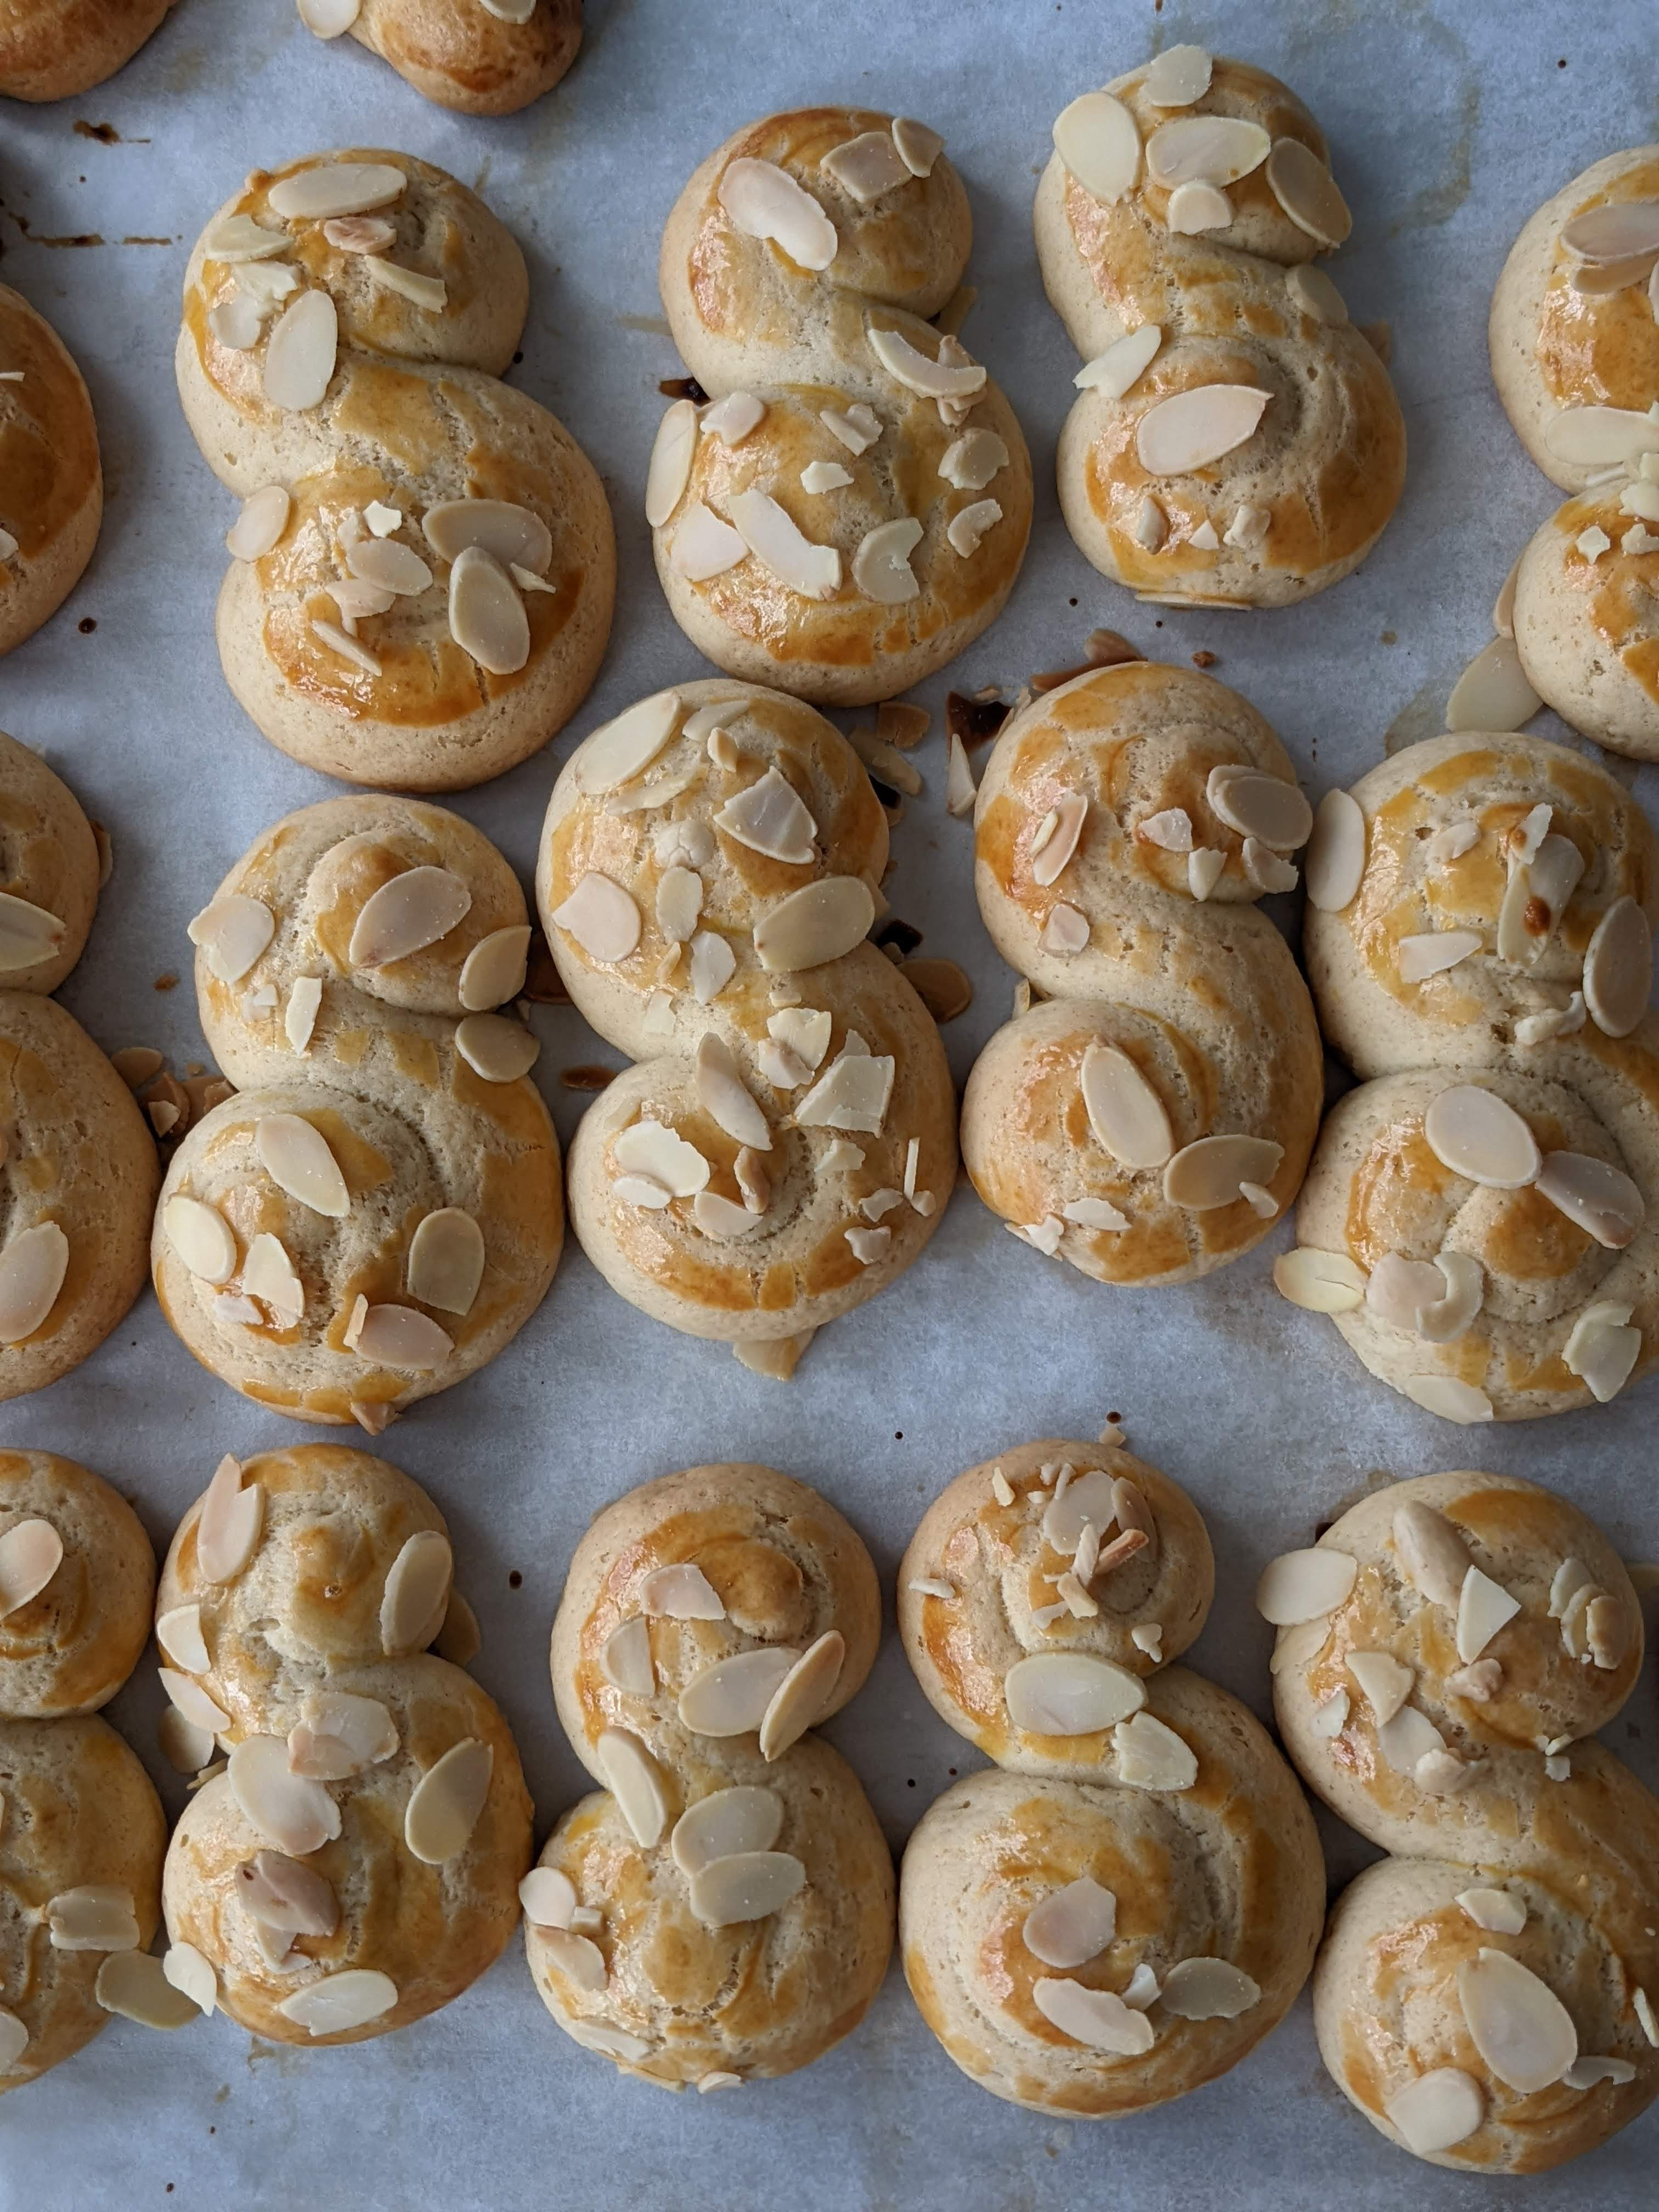
\includegraphics[width=60mm]{monanteras/images/Easter koulourakia.jpg}
% \end{figure}
%
% \begin{figure}
%   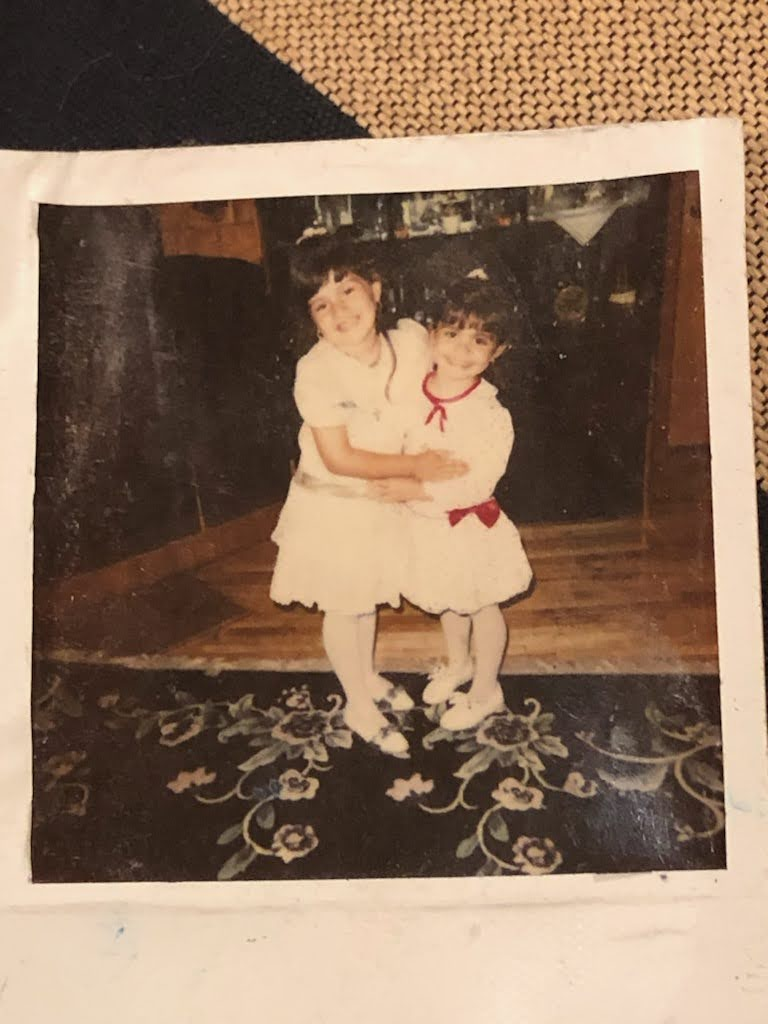
\includegraphics[width=60mm]{monanteras/images/IMG_20241009_171710.jpg}
%   \caption{Us in our Easter outfits, with our white Easter shoes}
% \end{figure}

\captionfigure{monanteras/images/IMG_20241009_171710.jpg}{Elsa and Helen in Easter outfits, with white Easter shoes!}{fig:easter_koulourakia_2}

